
This appendix gives an overview on consecutive steps applied while solving a heat conduction problem by means of a Finite Element Method. It is based on the the introductory course for FEM Modelling at ETH Zurich~\cite{eth_introduction_to_finite_element}. One can refer to this position to understand this topic in more details. Let us consider a partial differential equation of an unsteady one-dimensional heat conduction equation as 
\begin{equation}
    \frac{\partial T}{\partial t} = \frac{\partial}{\partial x} \left(k(x) \frac{\partial T}{\partial x} \right) + s(x), 
    \label{eqn:heat_conduction_pde}
\end{equation}
where $k(x)$ -- thermal conductivity as a function of space, $s(x)$ -- external heat source as a function of spaces. A temperature distribution is searched over the space and time, $T(x, t)$ that satisfies the given formula over the domain $\Omega \in \left[ 0, L \right]$. Two types of boundary conditions can be specified in the following problem: 
\begin{enumerate}
    \item 
    Dirichlet condition as \begin{equation}
    \left\{ \begin{array}{ lll }
    T(x_\text{A}, t) = T_\text{A},  \\ \\
    T(x_\text{B}, t) = T_\text{B},
    \end{array} \right.
    \end{equation}
    where $T_\text{A}$, $T_\text{B}$ -- constant temperatures at points A and B.
    
    \item Neumann condition as 
    \begin{equation}
    \left\{ \begin{array}{ lll }
    \left. k \frac{\partial T}{\partial x} \right|_{x=x_{\text{A},t}} = q_\text{A}, \\ \\
    \left. k \frac{\partial T}{\partial x} \right|_{x=x_{\text{B},t}} = q_\text{B},
    \end{array} \right.
    \label{eqn:neumann_bcs}
    \end{equation}
    where $q_\text{A}$ and $q_\text{A}$ heat flux at point A and B.
\end{enumerate}

In order to solve the equation being a function of time, the initial condition should be specified over the space as 
\begin{equation}
    T(x, t=0) = T_0(x).
\end{equation}

Discretisation involves a division of the analysed space into a finite number of elements consisting of nodes. Figure~\ref{fig:1d_element} shows a one-dimensional element with two nodes at its extremities. 

\begin{figure}[H]
    \centering
    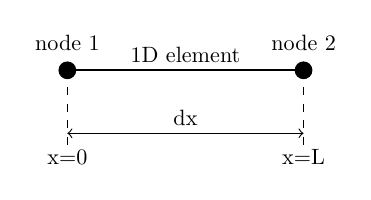
\begin{tikzpicture}[scale = 1]
        \filldraw[black] (0, 0) circle (3pt);
        \filldraw[black] (3, 0) circle (3pt);
        \draw[thick, black] (0, 0) -- (3, 0);
        \draw[thin, black, <->] (0, -0.8) -- (3, -0.8);
        \draw[thin, black, dashed] (0, 0) -- (0, -1);
        \draw[thin, black, dashed] (3, 0) -- (3, -1);
        \node[scale = 0.8] at (1.5, -0.6) {dx};
        \node[scale = 0.8] at (1.5, 0.2) {1D element};
        \node[scale = 0.8] at (0, 0.35) {node 1};
        \node[scale = 0.8] at (3, 0.35) {node 2};
        \node[scale = 0.8] at (0, -1.1) {x=0};
        \node[scale = 0.8] at (3, -1.1) {x=L};
    \end{tikzpicture}
    \caption{Exemplary one-dimensional 2-node element~\cite{eth_introduction_to_finite_element}.}
    \label{fig:1d_element}
\end{figure}

The more nodes is used in the element, the higher accuracy is obtained. However, the computing time increases as well. If two nodes are used for a 1D element, the temperature between them is interpolated linearly. The temperature over the longitudinal space is represented as
\begin{equation}
    T(x) \approx    
    \begin{bmatrix}  
    N_1(x) & N_2(x)    
    \end{bmatrix} 
    \begin{bmatrix}  
    T_1(x) \\  T_2(x) 
    \end{bmatrix} 
    = \vect{N} \vect{X}, 
    \label{eqn:linear_shape_function}
\end{equation}
where $N_1(x)$ and $N_2(x)$ -- the linear shape functions that allow for approximating the temperature over the continuous space. The shape functions can be reformulated as 
\begin{equation}
    \left\{ \begin{array}{ lll }
    N_1(x) = 1 - \frac{x}{L} \\ \\
    N_2(x) = \frac{x}{L},
    \end{array} \right.
    \label{eqn:shape_functions_representation}
\end{equation}
where $L$ -- length between two nodes in Fig.\ref{fig:1d_element}, $x$ -- spatial variable varying for $x \in [0, L]$. The shape functions are illustrated in Fig.~\ref{fig:linear_shape_functions}.

\begin{figure}[H]
    \centering
    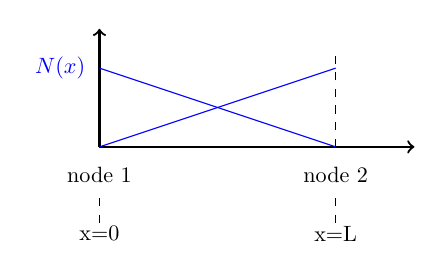
\begin{tikzpicture}[scale = 1]
    
        \draw[thick, black, ->] (0, 0) -- (4, 0);
        \draw[thick, black, ->] (0, 0) -- (0, 1.5);
        
        \draw[blue] (0, 0) -- (3, 1);
        \draw[blue] (0, 1) -- (3, 0);
        \node[scale = 0.8, blue] at (-0.5, 1) {$N(x)$};
        
        \draw[thin, black, dashed] (0, -0.65) -- (0, -1);
        \draw[thin, black, dashed] (3, -0.65) -- (3, -1);
        \draw[very thin, black, dashed] (3, 0) -- (3, 1.25);
    
        \node[scale = 0.8] at (0, -0.35) {node 1};
        \node[scale = 0.8] at (3, -0.35) {node 2};
        
        \node[scale = 0.8] at (0, -1.1) {x=0};
        \node[scale = 0.8] at (3, -1.1) {x=L};
    
    \end{tikzpicture}
    \caption{Representation of linear shape functions $N(x)$~\cite{eth_introduction_to_finite_element}.}
    \label{fig:linear_shape_functions}
\end{figure}

After substituting the approximated temperature distribution from (\ref{eqn:linear_shape_function}) to the differential equation from (\ref{eqn:heat_conduction_pde}), one obtains

\begin{equation}
     \frac{\partial}{\partial t} \left(   
     \begin{bmatrix}  
     N_1(x) & N_2(x)    
    \end{bmatrix} 
    \begin{bmatrix}  
    T_1(x) \\  T_2(x) 
    \end{bmatrix} \right) 
    - \frac{\partial}{\partial x} \left( k(x) \frac{\partial}{\partial x} \left( 
    \begin{bmatrix}  
    N_1(x) & N_2(x)    
    \end{bmatrix} 
    \begin{bmatrix}  
    T_1(x) \\  T_2(x) 
    \end{bmatrix} \right) \right) - s(x) = R,
    \label{eqn:residual_function}
\end{equation}
where $R$ -- a residual error being a result of the discretisation process. In the continuous solution, the residual is equal to zero. Equation~(\ref{eqn:residual_function}) still cannot be solved because the number of variables exceeds the number of equations. In order to solve this problem, Equation~(\ref{eqn:residual_function}) is multiplied by a set of so called "weighting functions". The weighted residual of such an expression must be equal to zero. One of the method, proposing a specific weighting function is called a Galerkin method. It is more explained in~\cite[p.~1-11]{eth_introduction_to_finite_element}.

In the next steps, the analysis is simplified by assuming the thermal conductivity and heat source independent of space. After applying the weighting functions, a set of algebraic equations is obtained as 

\begin{equation}
    \begin{bmatrix}  
    \frac{L}{3} & \frac{L}{6} \\
    \frac{L}{6} & \frac{L}{3}
    \end{bmatrix} 
    \begin{bmatrix}  
    \frac{\partial T_1}{\partial t} \\
    \frac{\partial T_2}{\partial t}
    \end{bmatrix} 
    + \bar k
    \begin{bmatrix}  
    \frac{1}{L} & -\frac{1}{L} \\
    -\frac{1}{L} & \frac{1}{L}
    \end{bmatrix} 
    \begin{bmatrix}  
    T_1 \\
    T_2
    \end{bmatrix} 
    = 
    \begin{bmatrix}  
    N_1 \left. q_\text{A} \right|_{x_\text{A}} \\
    N_2 \left. q_\text{A} \right|_{x_\text{A}}
    \end{bmatrix} 
    + \bar s 
    \begin{bmatrix}  
    \frac{L}{2} \\
    \frac{L}{2}
    \end{bmatrix},
    \label{eqn:set_algebraic_equations}
\end{equation}
where $\bar k$ -- constant thermal conductivity over each volume element $\left[x_\text{A}, x_\text{B} \right]$,  $\bar s$ -- constant heat source over the same element volume, $q_\text{A}$ -- heat flux at point A, $q_\text{B}$ -- heat flux at point B. In the derivation process, Neumann boundary conditions were assumed, as shown in~(\ref{eqn:neumann_bcs}). Equation~(\ref{eqn:set_algebraic_equations}) can be written in a matrix form as

\begin{equation}
    \vect{A} \frac{\partial \vect{T}}{\partial t} + \vect{B} \vect{T} = \vect{F},
\end{equation}
where 

\begin{equation}
    \vect{A} = 
    \begin{bmatrix}  
    \frac{L}{3} & \frac{L}{6} \\
    \frac{L}{6} & \frac{L}{3}
    \end{bmatrix},
\end{equation}

\begin{equation}
    \vect{B} = 
    \begin{bmatrix}  
    \frac{1}{L} & -\frac{1}{L} \\
    -\frac{1}{L} & \frac{1}{L}
    \end{bmatrix},
\end{equation}

\begin{equation}
    \vect{T} = 
    \begin{bmatrix}  
    T_1 \\
    T_2
    \end{bmatrix},
\end{equation}

\begin{equation}
    \vect{F} = 
    \begin{bmatrix}  
    N_1 \left. q_\text{A} \right|_{x_\text{A}} \\
    N_2 \left. q_\text{A} \right|_{x_\text{A}}
    \end{bmatrix} 
    + \bar s 
    \begin{bmatrix}  
    \frac{L}{2} \\
    \frac{L}{2}
    \end{bmatrix}.
\end{equation}

Since the problem is transient, one should discretise the temperature time derivative. A~finite difference method is used with an implicit discretisation as

\begin{equation}
    \vect{A} \frac{\vect{T}^{n+1} - \vect{T}^n}{\Delta t} + \vect{B} \vect{T}^{n+1} = \vect{F},
\end{equation}
where $\Delta t$ -- a time step between two iterations of the solution, $\vect{T}^n$ -- known temperature vector from the current iteration, $\vect{T}^{n+1}$ -- unknown temperature vector from the next iteration to compute. After rearranging the formula, one obtains
\begin{equation}
    \vect{K} \vect{T}^{n+1} =\vect{M} \vect{T}^{n} + \vect{F},
\end{equation}
where 
\begin{equation}
    \vect{K} = \frac{1}{\Delta t} \vect{A} + \vect{B},
\end{equation}

\begin{equation}
    \vect{M} = \frac{1}{\Delta t} \vect{A}.
\end{equation}

The matrix $\vect{K}$ is called the element stiffness matrix. While conducting a simulation with more degrees of freedom (DOF), i.e higher number of nodes, the stiffness matrices of every single element add up to form a large global stiffness matrix. The more DOF's are used, the more time consuming the problem becomes.